\documentclass{ximera}  


%\usepackage{todonotes}
%\usepackage{mathtools} %% Required for wide table Curl and Greens
%\usepackage{cuted} %% Required for wide table Curl and Greens
\newcommand{\todo}{}

\usepackage{esint} % for \oiint
\ifxake%%https://math.meta.stackexchange.com/questions/9973/how-do-you-render-a-closed-surface-double-integral
\renewcommand{\oiint}{{\large\bigcirc}\kern-1.56em\iint}
\fi


\graphicspath{
  {./}
  {jpg}
  {ximeraTutorial/}
  {basicPhilosophy/}
  {functionsOfSeveralVariables/}
  {normalVectors/}
  {lagrangeMultipliers/}
  {vectorFields/}
  {greensTheorem/}
  {shapeOfThingsToCome/}
  {dotProducts/}
  {partialDerivativesAndTheGradientVector/}
  {../productAndQuotientRules/exercises/}
  {../motionAndPathsInSpace/exercises/}
  {../normalVectors/exercisesParametricPlots/}
  {../continuityOfFunctionsOfSeveralVariables/exercises/}
  {../partialDerivativesAndTheGradientVector/exercises/}
  {../directionalDerivativeAndChainRule/exercises/}
  {../commonCoordinates/exercisesCylindricalCoordinates/}
  {../commonCoordinates/exercisesSphericalCoordinates/}
  {../greensTheorem/exercisesCurlAndLineIntegrals/}
  {../greensTheorem/exercisesDivergenceAndLineIntegrals/}
  {../shapeOfThingsToCome/exercisesDivergenceTheorem/}
  {../greensTheorem/}
  {../shapeOfThingsToCome/}
  {../separableDifferentialEquations/exercises/}
  {vectorFields/}
}

\newcommand{\mooculus}{\textsf{\textbf{MOOC}\textnormal{\textsf{ULUS}}}}

\usepackage{tkz-euclide}\usepackage{tikz}
\usepackage{tikz-cd}
\usetikzlibrary{arrows}
\tikzset{>=stealth,commutative diagrams/.cd,
  arrow style=tikz,diagrams={>=stealth}} %% cool arrow head
\tikzset{shorten <>/.style={ shorten >=#1, shorten <=#1 } } %% allows shorter vectors

\usetikzlibrary{backgrounds} %% for boxes around graphs
\usetikzlibrary{shapes,positioning}  %% Clouds and stars
\usetikzlibrary{matrix} %% for matrix
\usepgfplotslibrary{polar} %% for polar plots
\usepgfplotslibrary{fillbetween} %% to shade area between curves in TikZ
\usetkzobj{all}
\usepackage[makeroom]{cancel} %% for strike outs
%\usepackage{mathtools} %% for pretty underbrace % Breaks Ximera
%\usepackage{multicol}
\usepackage{pgffor} %% required for integral for loops



%% http://tex.stackexchange.com/questions/66490/drawing-a-tikz-arc-specifying-the-center
%% Draws beach ball
\tikzset{pics/carc/.style args={#1:#2:#3}{code={\draw[pic actions] (#1:#3) arc(#1:#2:#3);}}}



\usepackage{array}
\setlength{\extrarowheight}{+.1cm}
\newdimen\digitwidth
\settowidth\digitwidth{9}
\def\divrule#1#2{
\noalign{\moveright#1\digitwidth
\vbox{\hrule width#2\digitwidth}}}





\newcommand{\RR}{\mathbb R}
\newcommand{\R}{\mathbb R}
\newcommand{\N}{\mathbb N}
\newcommand{\Z}{\mathbb Z}

\newcommand{\sagemath}{\textsf{SageMath}}


%\renewcommand{\d}{\,d\!}
\renewcommand{\d}{\mathop{}\!d}
\newcommand{\dd}[2][]{\frac{\d #1}{\d #2}}
\newcommand{\pp}[2][]{\frac{\partial #1}{\partial #2}}
\renewcommand{\l}{\ell}
\newcommand{\ddx}{\frac{d}{\d x}}

\newcommand{\zeroOverZero}{\ensuremath{\boldsymbol{\tfrac{0}{0}}}}
\newcommand{\inftyOverInfty}{\ensuremath{\boldsymbol{\tfrac{\infty}{\infty}}}}
\newcommand{\zeroOverInfty}{\ensuremath{\boldsymbol{\tfrac{0}{\infty}}}}
\newcommand{\zeroTimesInfty}{\ensuremath{\small\boldsymbol{0\cdot \infty}}}
\newcommand{\inftyMinusInfty}{\ensuremath{\small\boldsymbol{\infty - \infty}}}
\newcommand{\oneToInfty}{\ensuremath{\boldsymbol{1^\infty}}}
\newcommand{\zeroToZero}{\ensuremath{\boldsymbol{0^0}}}
\newcommand{\inftyToZero}{\ensuremath{\boldsymbol{\infty^0}}}



\newcommand{\numOverZero}{\ensuremath{\boldsymbol{\tfrac{\#}{0}}}}
\newcommand{\dfn}{\textbf}
%\newcommand{\unit}{\,\mathrm}
\newcommand{\unit}{\mathop{}\!\mathrm}
\newcommand{\eval}[1]{\bigg[ #1 \bigg]}
\newcommand{\seq}[1]{\left( #1 \right)}
\renewcommand{\epsilon}{\varepsilon}
\renewcommand{\phi}{\varphi}


\renewcommand{\iff}{\Leftrightarrow}

\DeclareMathOperator{\arccot}{arccot}
\DeclareMathOperator{\arcsec}{arcsec}
\DeclareMathOperator{\arccsc}{arccsc}
\DeclareMathOperator{\si}{Si}
\DeclareMathOperator{\scal}{scal}
\DeclareMathOperator{\sign}{sign}


%% \newcommand{\tightoverset}[2]{% for arrow vec
%%   \mathop{#2}\limits^{\vbox to -.5ex{\kern-0.75ex\hbox{$#1$}\vss}}}
\newcommand{\arrowvec}[1]{{\overset{\rightharpoonup}{#1}}}
%\renewcommand{\vec}[1]{\arrowvec{\mathbf{#1}}}
\renewcommand{\vec}[1]{{\overset{\boldsymbol{\rightharpoonup}}{\mathbf{#1}}}\hspace{0in}}

\newcommand{\point}[1]{\left(#1\right)} %this allows \vector{ to be changed to \vector{ with a quick find and replace
\newcommand{\pt}[1]{\mathbf{#1}} %this allows \vec{ to be changed to \vec{ with a quick find and replace
\newcommand{\Lim}[2]{\lim_{\point{#1} \to \point{#2}}} %Bart, I changed this to point since I want to use it.  It runs through both of the exercise and exerciseE files in limits section, which is why it was in each document to start with.

\DeclareMathOperator{\proj}{\mathbf{proj}}
\newcommand{\veci}{{\boldsymbol{\hat{\imath}}}}
\newcommand{\vecj}{{\boldsymbol{\hat{\jmath}}}}
\newcommand{\veck}{{\boldsymbol{\hat{k}}}}
\newcommand{\vecl}{\vec{\boldsymbol{\l}}}
\newcommand{\uvec}[1]{\mathbf{\hat{#1}}}
\newcommand{\utan}{\mathbf{\hat{t}}}
\newcommand{\unormal}{\mathbf{\hat{n}}}
\newcommand{\ubinormal}{\mathbf{\hat{b}}}

\newcommand{\dotp}{\bullet}
\newcommand{\cross}{\boldsymbol\times}
\newcommand{\grad}{\boldsymbol\nabla}
\newcommand{\divergence}{\grad\dotp}
\newcommand{\curl}{\grad\cross}
%\DeclareMathOperator{\divergence}{divergence}
%\DeclareMathOperator{\curl}[1]{\grad\cross #1}
\newcommand{\lto}{\mathop{\longrightarrow\,}\limits}

\renewcommand{\bar}{\overline}

\colorlet{textColor}{black}
\colorlet{background}{white}
\colorlet{penColor}{blue!50!black} % Color of a curve in a plot
\colorlet{penColor2}{red!50!black}% Color of a curve in a plot
\colorlet{penColor3}{red!50!blue} % Color of a curve in a plot
\colorlet{penColor4}{green!50!black} % Color of a curve in a plot
\colorlet{penColor5}{orange!80!black} % Color of a curve in a plot
\colorlet{penColor6}{yellow!70!black} % Color of a curve in a plot
\colorlet{fill1}{penColor!20} % Color of fill in a plot
\colorlet{fill2}{penColor2!20} % Color of fill in a plot
\colorlet{fillp}{fill1} % Color of positive area
\colorlet{filln}{penColor2!20} % Color of negative area
\colorlet{fill3}{penColor3!20} % Fill
\colorlet{fill4}{penColor4!20} % Fill
\colorlet{fill5}{penColor5!20} % Fill
\colorlet{gridColor}{gray!50} % Color of grid in a plot

\newcommand{\surfaceColor}{violet}
\newcommand{\surfaceColorTwo}{redyellow}
\newcommand{\sliceColor}{greenyellow}




\pgfmathdeclarefunction{gauss}{2}{% gives gaussian
  \pgfmathparse{1/(#2*sqrt(2*pi))*exp(-((x-#1)^2)/(2*#2^2))}%
}


%%%%%%%%%%%%%
%% Vectors
%%%%%%%%%%%%%

%% Simple horiz vectors
\renewcommand{\vector}[1]{\left\langle #1\right\rangle}


%% %% Complex Horiz Vectors with angle brackets
%% \makeatletter
%% \renewcommand{\vector}[2][ , ]{\left\langle%
%%   \def\nextitem{\def\nextitem{#1}}%
%%   \@for \el:=#2\do{\nextitem\el}\right\rangle%
%% }
%% \makeatother

%% %% Vertical Vectors
%% \def\vector#1{\begin{bmatrix}\vecListA#1,,\end{bmatrix}}
%% \def\vecListA#1,{\if,#1,\else #1\cr \expandafter \vecListA \fi}

%%%%%%%%%%%%%
%% End of vectors
%%%%%%%%%%%%%

%\newcommand{\fullwidth}{}
%\newcommand{\normalwidth}{}



%% makes a snazzy t-chart for evaluating functions
%\newenvironment{tchart}{\rowcolors{2}{}{background!90!textColor}\array}{\endarray}

%%This is to help with formatting on future title pages.
\newenvironment{sectionOutcomes}{}{}



%% Flowchart stuff
%\tikzstyle{startstop} = [rectangle, rounded corners, minimum width=3cm, minimum height=1cm,text centered, draw=black]
%\tikzstyle{question} = [rectangle, minimum width=3cm, minimum height=1cm, text centered, draw=black]
%\tikzstyle{decision} = [trapezium, trapezium left angle=70, trapezium right angle=110, minimum width=3cm, minimum height=1cm, text centered, draw=black]
%\tikzstyle{question} = [rectangle, rounded corners, minimum width=3cm, minimum height=1cm,text centered, draw=black]
%\tikzstyle{process} = [rectangle, minimum width=3cm, minimum height=1cm, text centered, draw=black]
%\tikzstyle{decision} = [trapezium, trapezium left angle=70, trapezium right angle=110, minimum width=3cm, minimum height=1cm, text centered, draw=black]




 
\title{Impedance and Admittance on Smith Chart} 
\author{Milica Markovic} 
\outcome{Read normalized impedance and reflection coefficient on the Smith Chart given a random point on the Smith Chart. Given impedance, find the normalized position of the impedance on the Smith Chart. Describe the reason for introducing admittance. Write the impedance and admittance of an inductor and capacitor. Explain why is the susceptance of an inductor negative and reactance is positive. Explain why is the admittance Smith Chart rotated 180 degrees. Distinguish between load impedance and normalized load impedance. Describe impedances on the Smith Chart as normalized impedances.Given impedance, read admittance on combo Y/Z chart. Given a random point on Y/Z chart, find admittance, impedance and the reflection coefficient.}
\begin{document}  
\begin{abstract}  

\end{abstract}  
\maketitle    




\section{Brief review of impedance and admittance}

Impedance's $Z =R+jX$real part is called resistance $R$, and the imaginary part is called reactance $X$. It is easier to add impedances when elements are in series; see Figure \ref{fig:SCDerimpadmtrans}. To find the total impedance, we add resistances and reactances separately. 

 The real part of an admittance $Y=G+jB$  is called conductance G, and the imaginary part is called susceptance B. It is easier to add admittances when elements are in parallel; see Figure \ref{fig:SCDerimpadmtrans}. When adding two admittances, we add conductances and susceptances separately.  
 
\begin{figure}[htbp]
\begin{center}
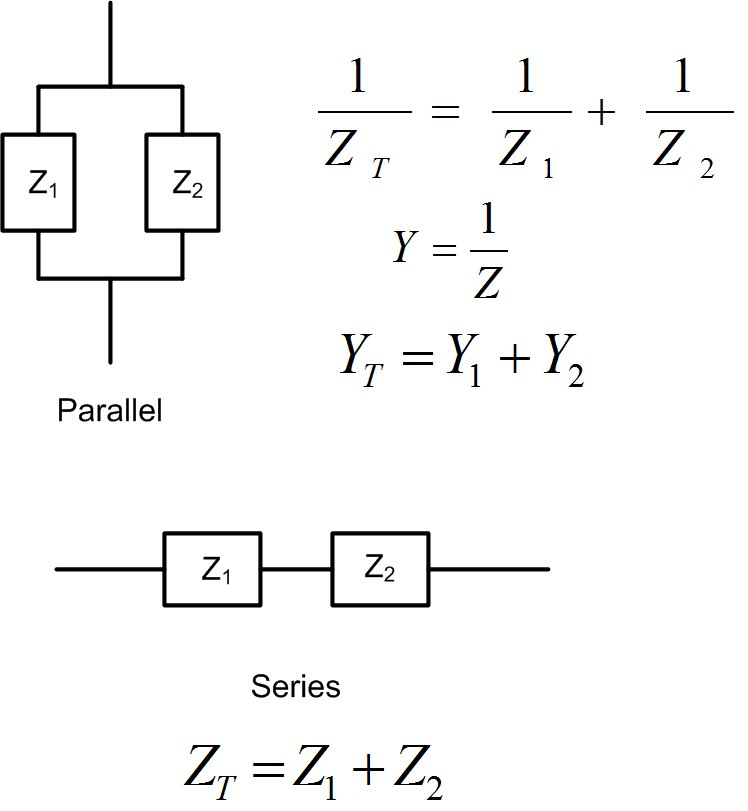
\includegraphics[scale=0.25]{../jpg/Impedance_Admittance.jpg}
\end{center}
\caption{It is easier to use admittance when the circuit elements are in parallel and impedance when the circuit elements are in series.}
\label{fig:SCDerimpadmtrans}
\end{figure}


 Smith Chart in Figure \ref{fig:SCDerscadmimp} has impedance  circles, and impedance coordinates on it.  We can use this Smith Chart to read off the values for the impedance, and reflection coefficient. In the next section, we will learn to use impedance/admittance (Z/Y) Smith Chart, where both impedance and admittance circles are shown. We will use the Z/Y Smith Chart when we add impedances or admittances in parallel or series, which is useful in impedance matching that we will talk about in the next chapter. 


\begin{figure}[htbp]
\begin{center}
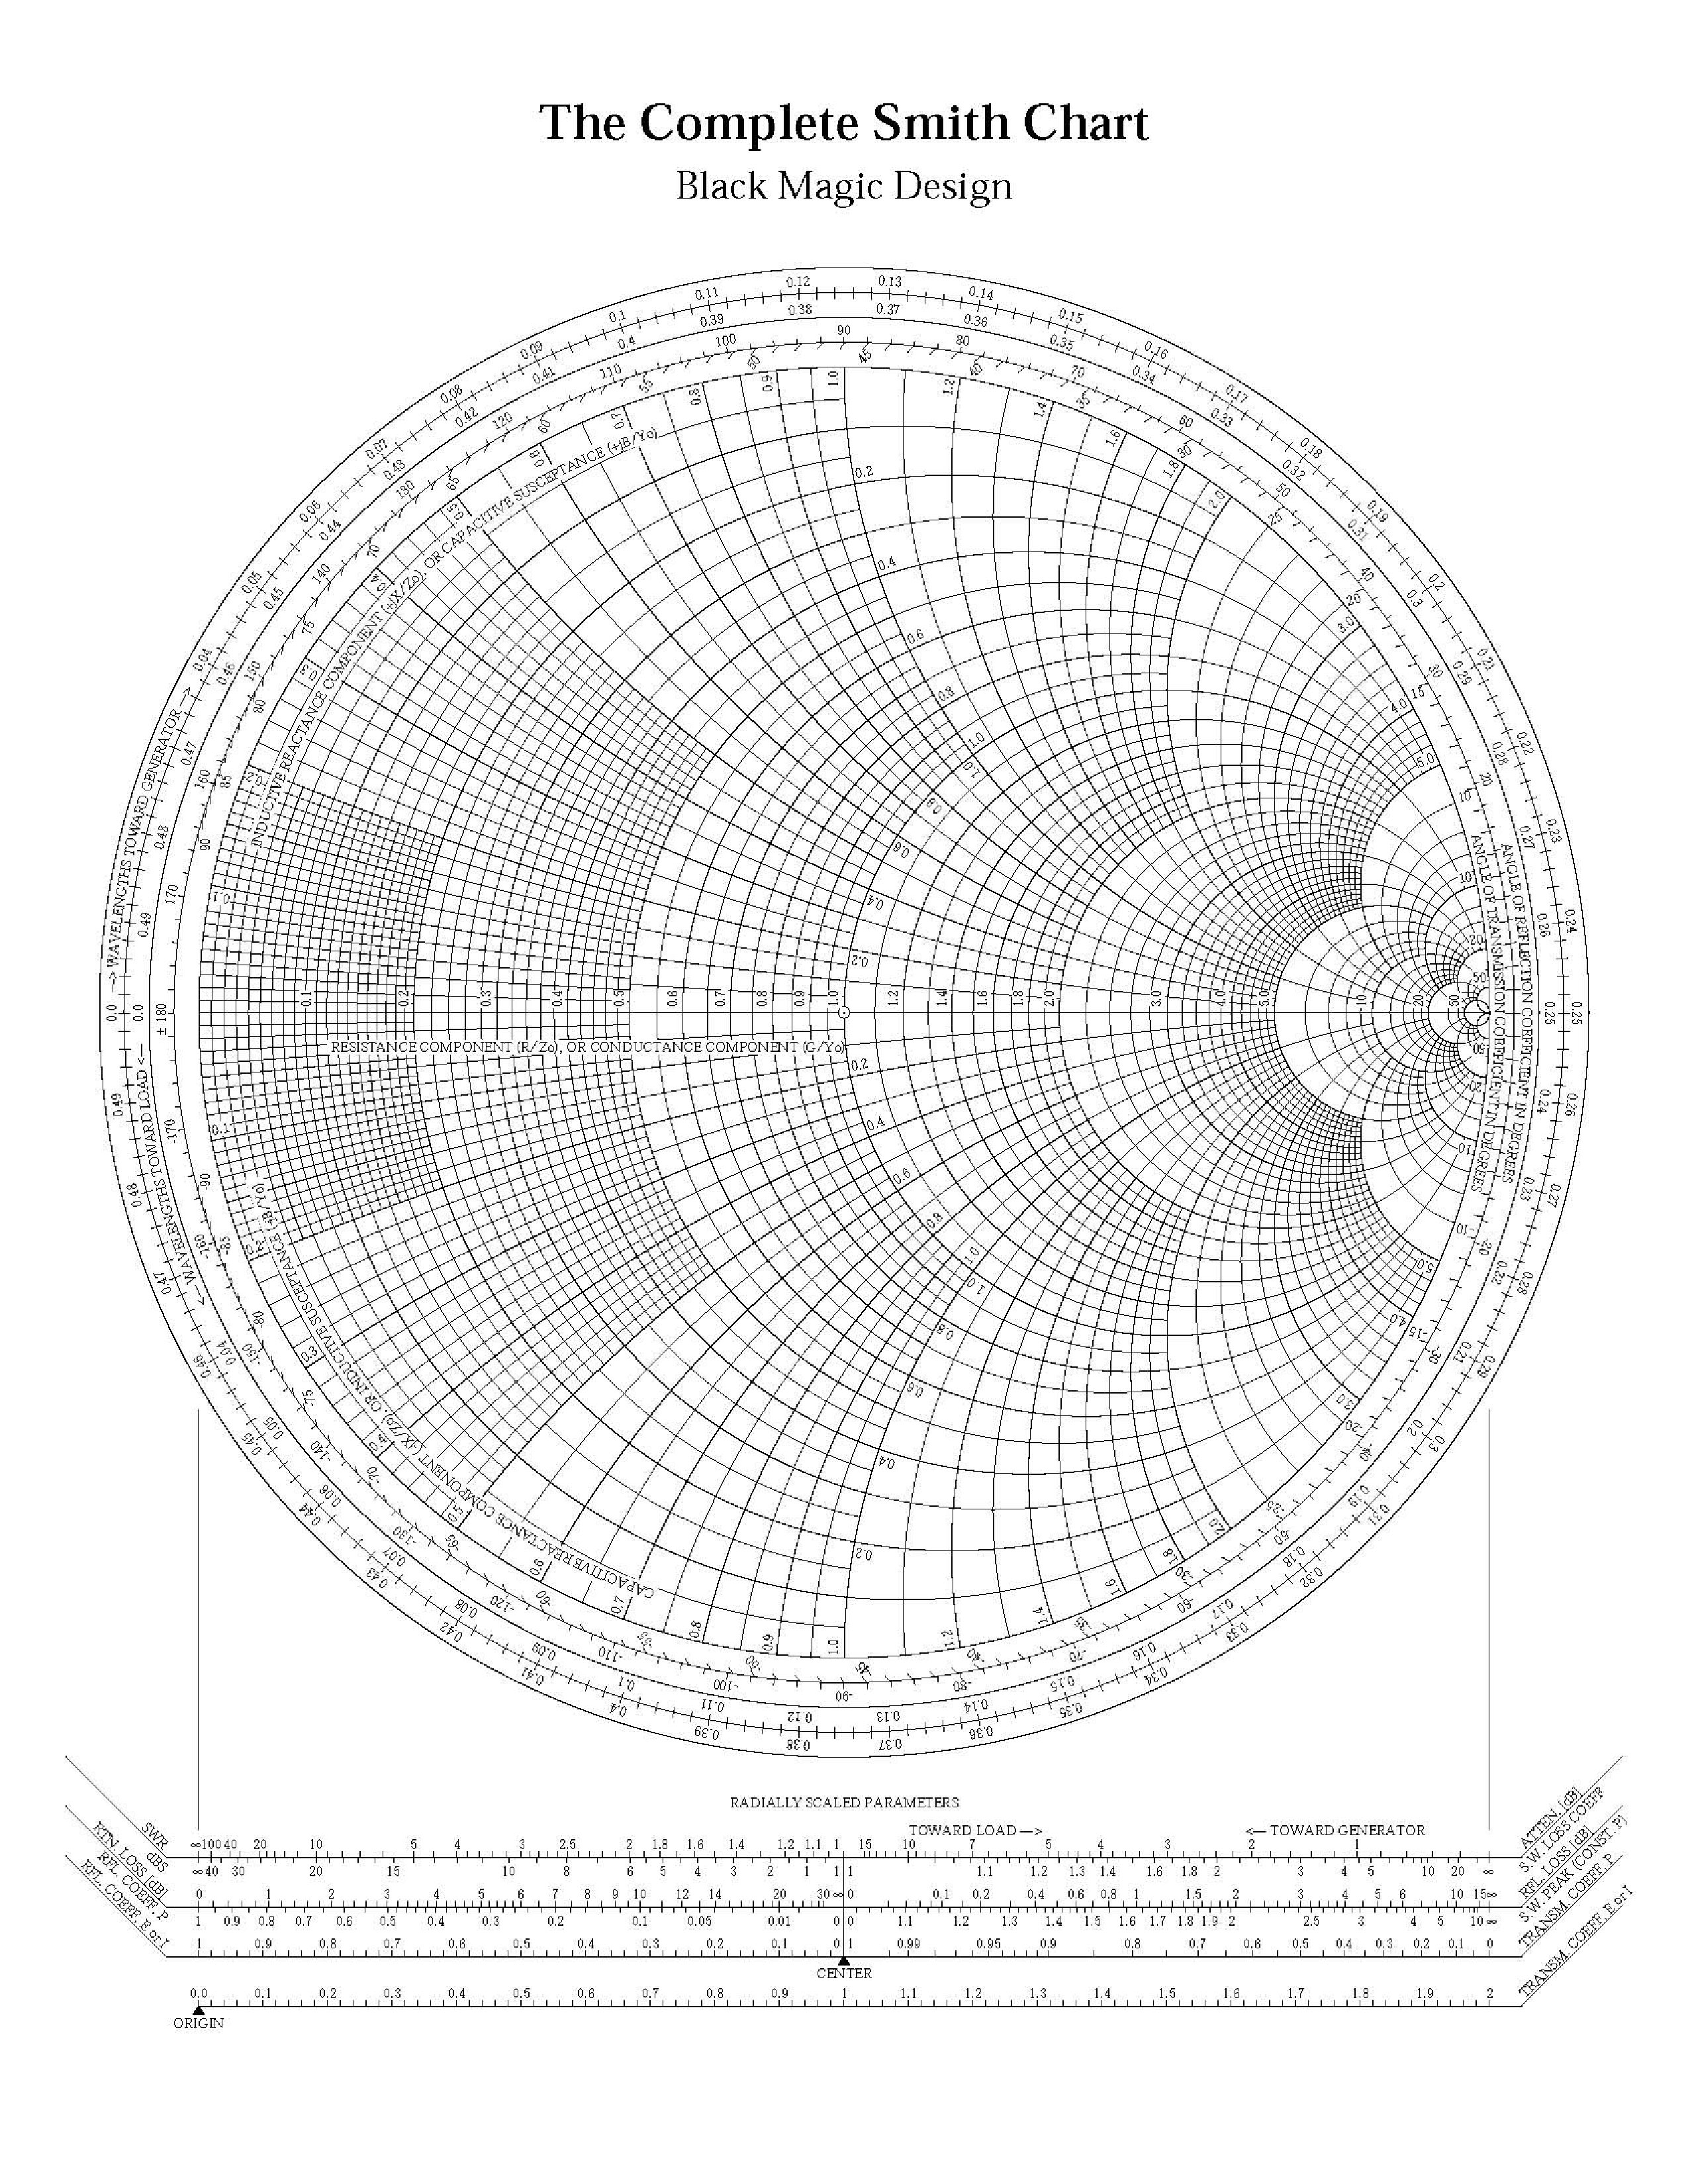
\includegraphics[scale=0.1]{../jpg/SmithChartImped-01.jpg}
\end{center}
\caption{On Smith Chart impedances are shown in red, and admittances in green.}
\label{fig:SCDerscadmimp}
\end{figure}



\section{Impedance on the Smith Chart} 

Figure \ref{fig:SCDerscimpedance}, shows how to find the location of normalized impedance  $z_L=1+j 1$ on the Smith Chart.  $z_L=1+j 1$ is at a point where the circle of constant resistance $r_L=1$ crosses the circle of constant reactance $x_L=1$.   Figure \ref{fig:SCDerscgammafromZ} shows how to find the reflection coefficient if normalized load impedance $z_L=1+j 1$ is given. Measure the distance between the origin and the point using the scale "Reflection Coefficient E or I" on the Smith Chart's bottom to find the reflection coefficient's magnitude. To find the reflection coefficient's angle, we read the scale "Angle of Reflection Coefficient" on the Smith Chart's perimeter, shown in green. The reflection coefficient is therefore $0.5 e^{j 62^o}$, which is close to the actual value   $0.5 e^{j 64^o}$. If we use a ruler and compass, and a nicely sharpened pencil, we will get exactly the right answer. Try it out!


\begin{figure}[htbp]
\begin{center}
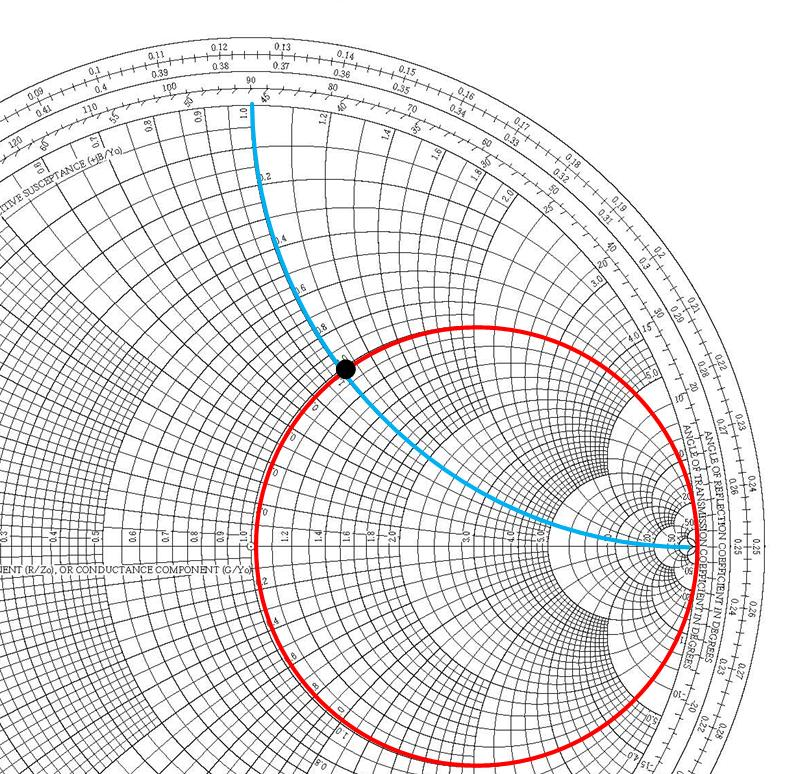
\includegraphics[scale=0.3]{../jpg/FindingImpedanceonSC.jpg}
\end{center}
\caption{Red circle that represents all points on Smith Chart with normalized resistance $r=1$ and blue circle that represents all points on Smith Chart with  normalized reactance $x=1$ cross at point where $Z_L=1+j 1$.}
\label{fig:SCDerscimpedance}
\end{figure}

\begin{figure}[htbp]
\begin{center}
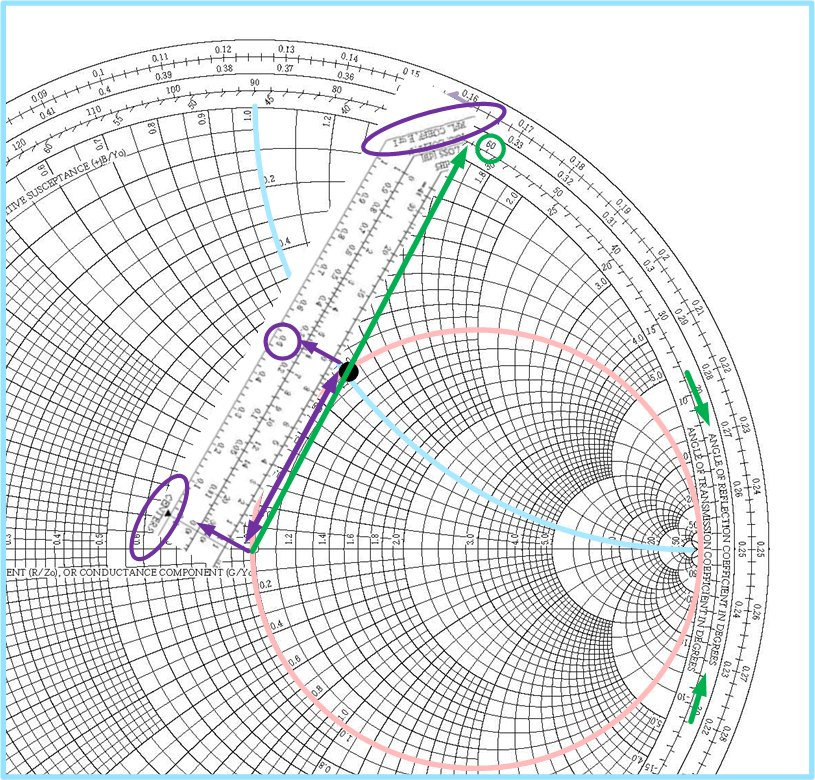
\includegraphics[scale=0.3]{../jpg/FindingGammaFromImpedanceonSC.jpg}
\end{center}
\caption{To find the magnitude of the reflection coefficient from impedance $Z_L=1+j 1$, we measure the distance between the origin and the point using the scale "Reflection Coefficient E or I" on the bottom of the Smith Chart. To find the reflection coefficient's angle, we read the scale "Angle of Reflection Coefficient" on the perimeter of the Smith Chart.}
\label{fig:SCDerscgammafromZ}
\end{figure}


\newpage

\section{Admittance on the impedance Smith Chart} 

The reflection coefficient can be found from impedance or admittance. To find the reflection coefficient from impedance, we use the formula that we previously derived, where $Z_L$ is the load impedance, and $z_L=\frac{Z_L}{Z_0}$ is the normalized load impedance.

\begin{eqnarray}
\Gamma_L=\frac{z_L-1}{z_L+1} \label{eq:GammaImp} 
\end{eqnarray}


Admittance is defined as $Y_L=\frac{1}{Z_L}$, and the transmission-line admittance is defined as $Y_0=\frac{1}{Z_0}$. If we now replace the impedances in the equation above with admittances, we get


\begin{eqnarray}
\Gamma_L = \frac{\frac{1}{Y_L}-\frac{1}{Y_0}}{\frac{1}{Y_L}+\frac{1}{Y_0}} \\
\Gamma_L = \frac{Y_0-Y_L}{Y_0+Y_L} \\
\Gamma_L = -  \frac{Y_L-Y_0}{Y_L+Y_0} \\
\Gamma_L = -  \frac{y_L-1}{y_L+1} \\
\Gamma_L = -\Gamma_Y \label{eq:GammaAdm}
\end{eqnarray}


Where $Y_L$ is the load admittance and $y_L=\frac{Y_L}{Y_0} $, is the normalized load admittance. Note that the Smith Chart shown in Figure \ref{fig:SCDerscimpedance} shows circles for the impedance of the load. Therefore, the true reflection coefficient of the load is at the position of the load. We have defined $\Gamma_Y $ above to see the position of admittance on the impedance Smith Chart. 


 From the above Equation \ref{eq:GammaAdm}, we can see that the reflection coefficient for the admittance (and the admittance) on the impedance Smith chart has the same magnitude as the load reflection coefficient. The $\Gamma_Y$ is on the same SWR circle as the $\Gamma_L$, but it is $180^0$ shifted with respect to the load reflection coefficient. $180^0$ phase shift in reflection coefficient with the same magnitude can be found in two ways:
 
\begin{enumerate}
\item  by rotating the reflection coefficient $\Gamma_L$ for $180^0$ on the SWR circle to read the admittance of the load. Effectively, this means that you can draw a line through the load impedance and the center of the Smith Chart, and find the position of this line that crosses the SWR circle, $180^0$ away. This method's disadvantage is that the point representing admittance changes place on the Smith Chart, depending on whether we are reading admittance or impedance. This method is used in some books, see, for example, Ulaby, Applied Electromagnetics.

\item Another way to read the admittances on the Smith chart is to use combination of impedance/admittance (Z/I) chart, Figure \ref{fig:SCDerscadmimp1}. To make the Z/Y chart, we rotate the impedance Smith Chart for $180^0$ to get the admittance point at the same position as the impedance point. Then, the impedance, admittance, and reflection coefficient are all at the same point, but we have to read the two scales, the impedance and admittance scale. The disadvantage of this method is that the Z/Y Smith Chart has more circles to read. However, this method is conceptually more straightforward, as the point on the Smith Chart does not change position, depending on whether we are reading admittance or impedance. The point is fixed, and we just read the different circles. We will use this method in our class. The example below discusses this method further.


\begin{figure}[htbp]
\begin{center}
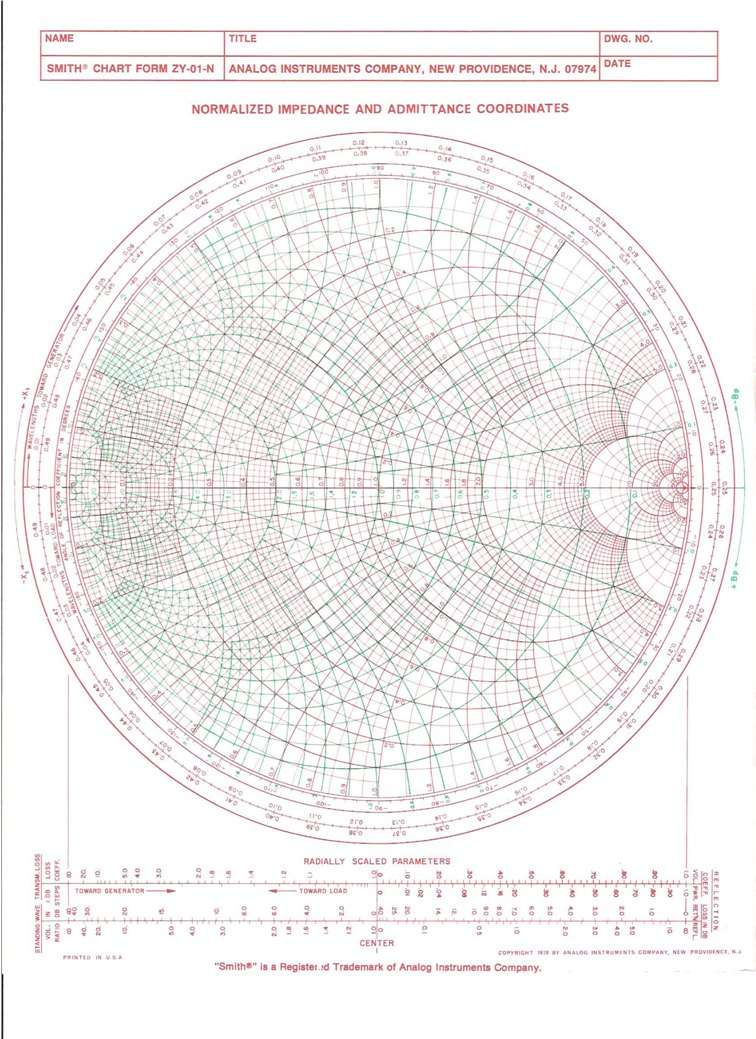
\includegraphics[scale=0.3]{../jpg/SCadmimp.jpg}
\end{center}
\caption{On Z/Y Smith Chart impedances are shown in red, and admittances in green.}
\label{fig:SCDerscadmimp1}
\end{figure}

\end{enumerate} 
 




\begin{example}
The normalized impedance of the load is given $z_L=1+j1$. First, find the admittance of this impedance using your calculator. Then use two Smith Charts. On one, find the impedance position, and on the other, find the position of the admittance. Then rotate the admittance chart for $180^0$ so that both points overlap. Observe the impedance and admittance circles on this combo Z/Y chart, and compare them to the Z/Y chart.

\begin{solution}
The normalized admittance to impedance  $z_L=1+j1$ is $y_L=0.5-j0.5$.

\end{solution}

The impedance $z_L=1+j1$ is shown on the Smith Chart in Figure \ref{fig:SC1-imp}.

\begin{figure}[htbp]
\begin{center}
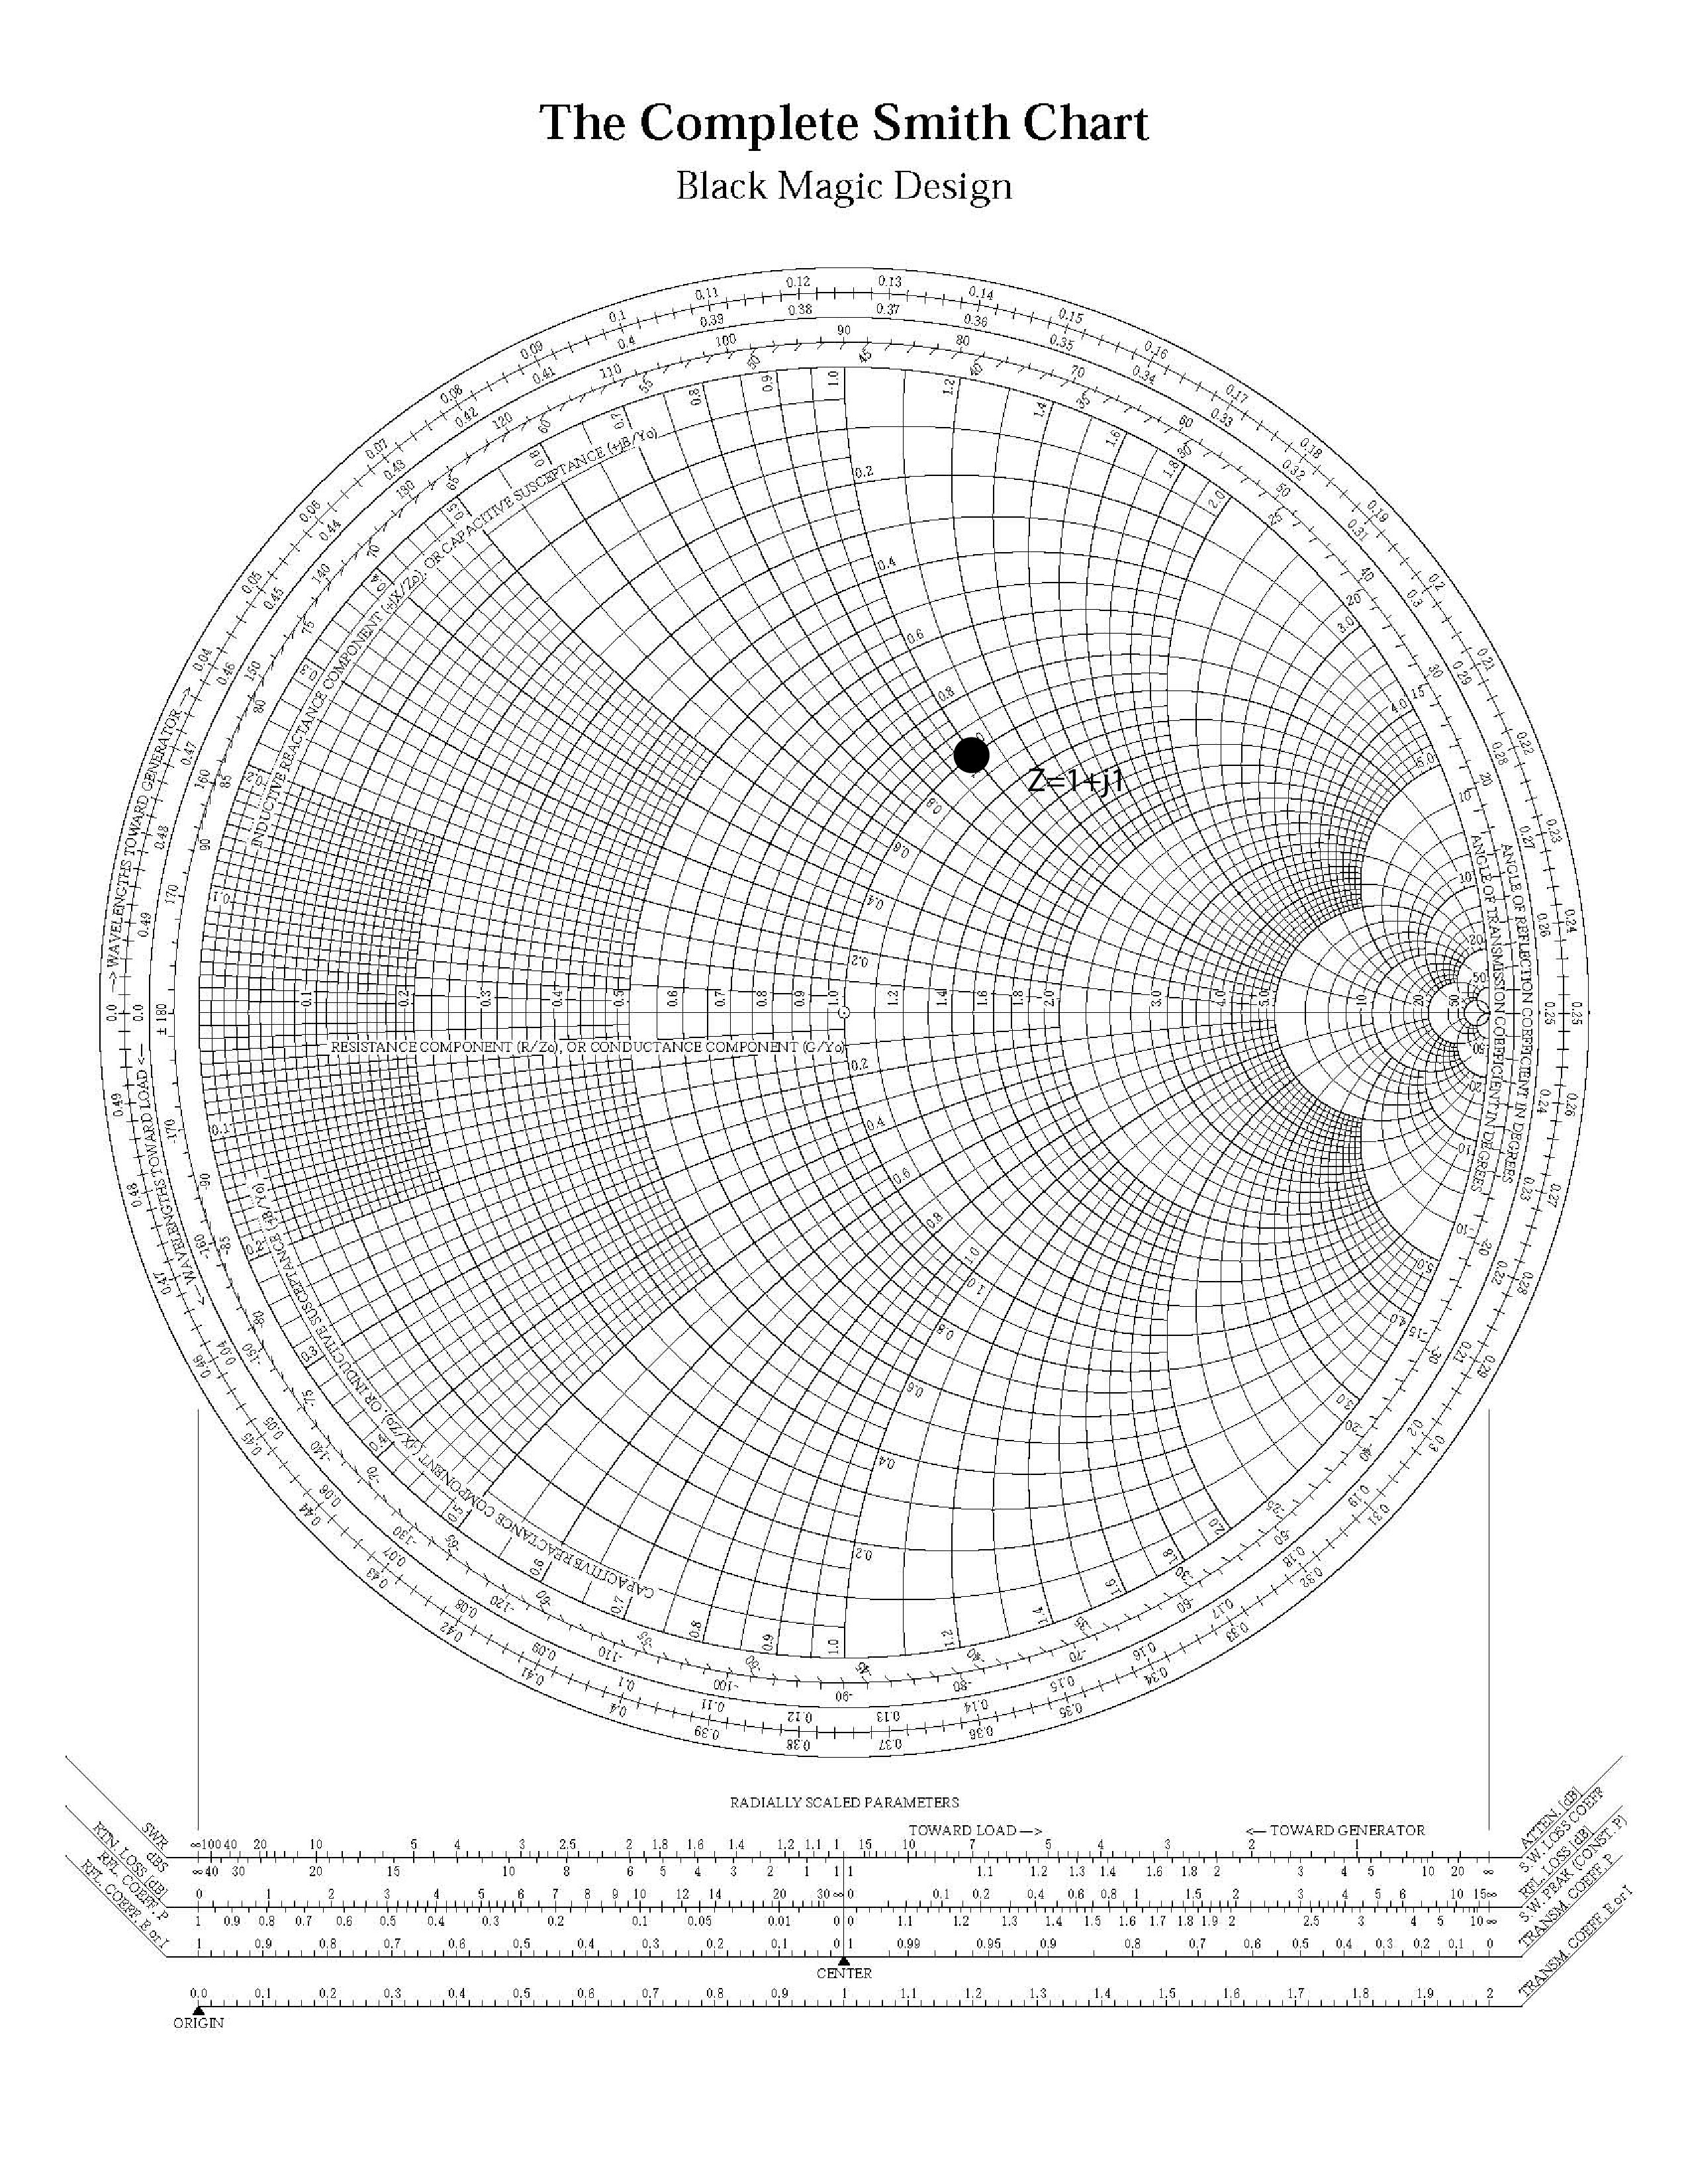
\includegraphics[scale=0.1]{../jpg/Zchart-01-01.jpg}
\end{center}
\caption{Impedance $z_L=1+j1$ on Smith Chart} \label{fig:SC1-imp}
\end{figure}

The admittance $y_L=0.5-j0.5$ is shown on Smith Chart in Figure \ref{fig:SC1-adm}. If we now use this Smith Chart and rotate it for $180^0$ (upside down), and place it over the chart above, we will see that the impedance and admittance point are in the same position on the Smith Chart. We call this Smith Chart a z/y Smith Chart. 

\begin{figure}[htbp]
\begin{center}
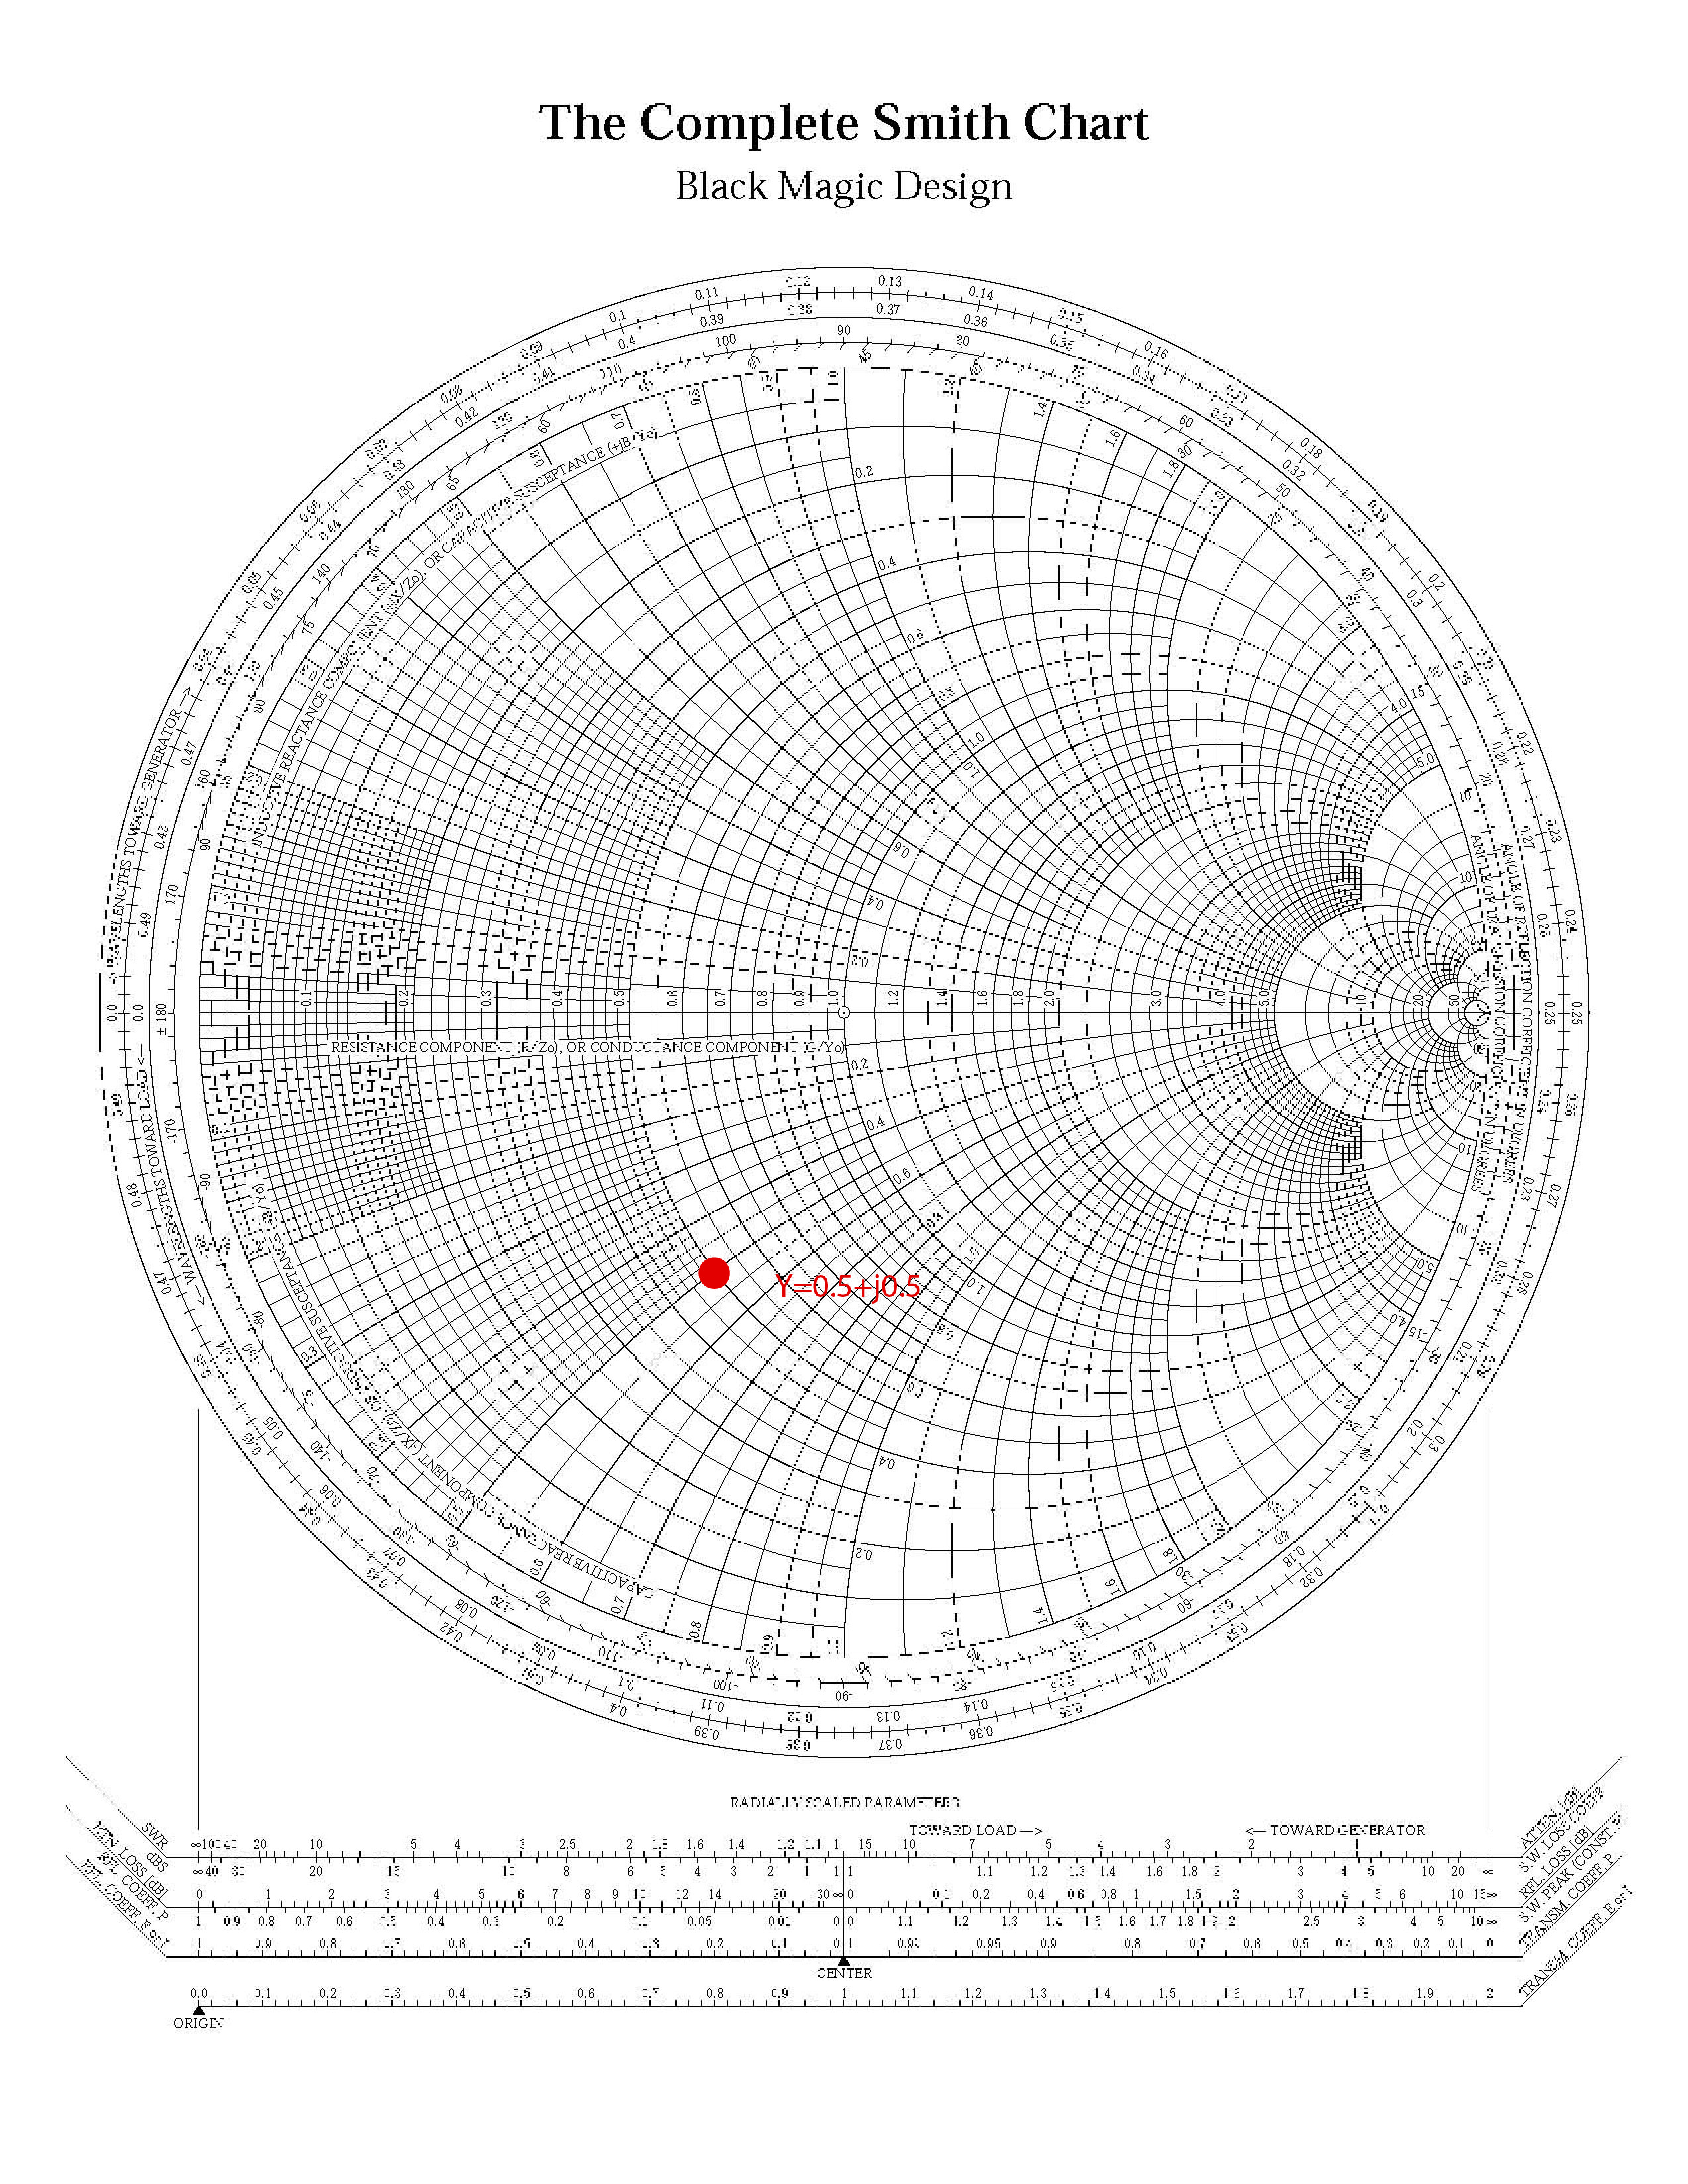
\includegraphics[scale=0.1]{../jpg/Ychart-01.jpg}
\end{center}
\caption{Admittance $y_L=0.5-j0.5$ on Smith Chart} \label{fig:SC1-adm}
\end{figure}


Both impedance  $z_L=1+j1$ and admittance $y_L=0.5-j0.5$ are at the same position on the z/y Smith Chart in Figure \ref{fig:SC1-both}. We see two sets of circles on this chart, the red ones represent impedance circles, and the green ones represent admittance circles. To read the impedance of the point shown on the Smith Chart, we read the impedance circle scale, and to read the admittance, we read the admittance circle scales.


\begin{figure}[htbp]
\begin{center}
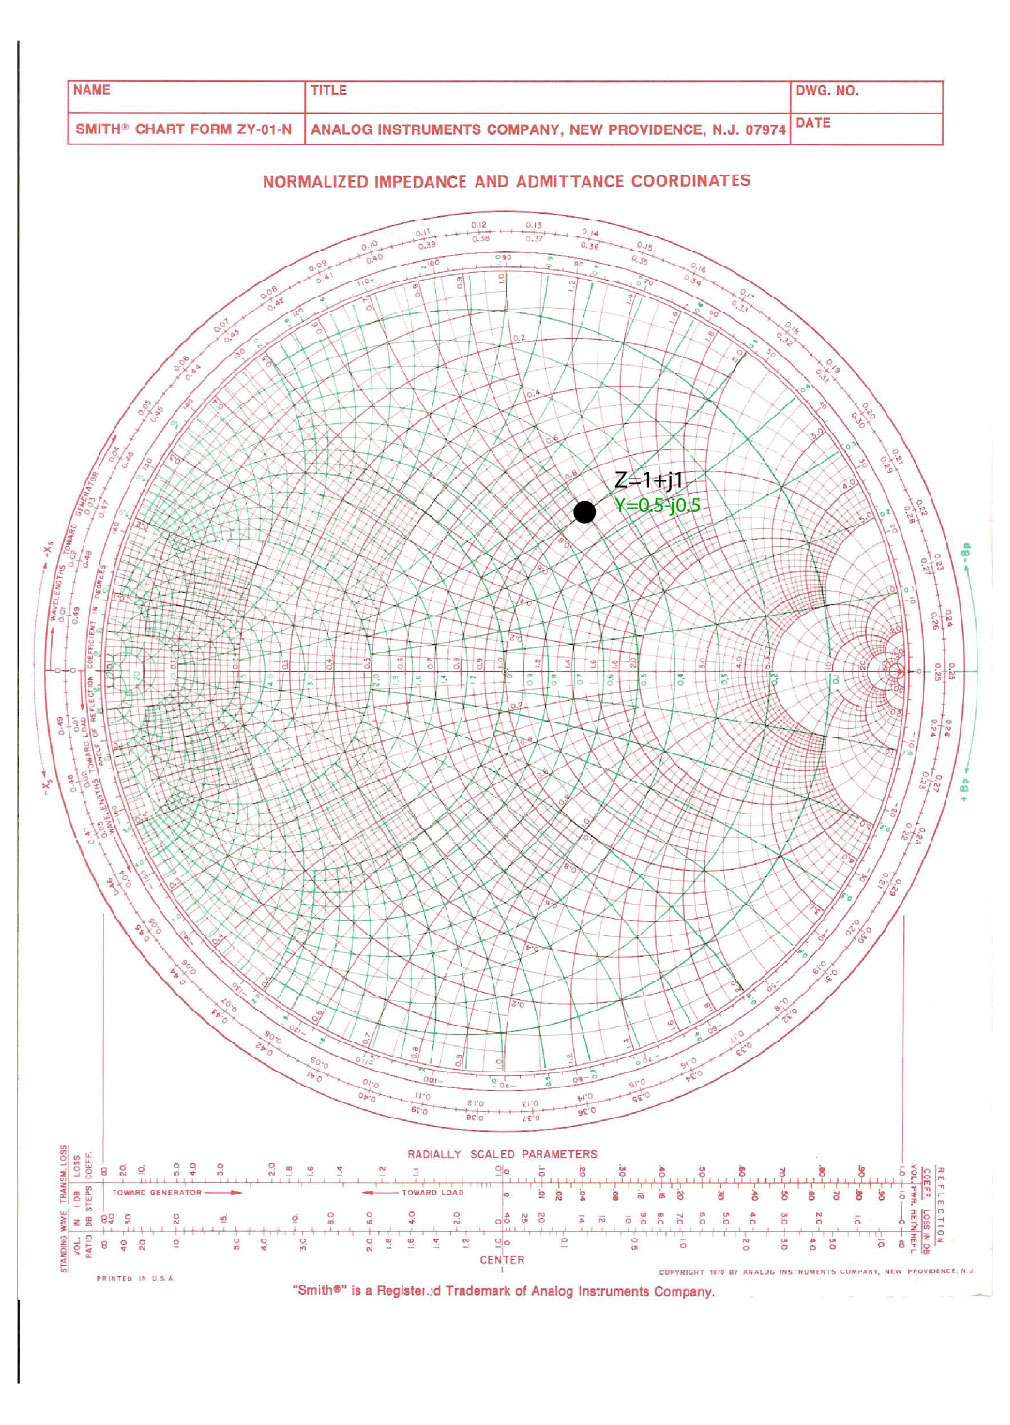
\includegraphics[scale=1]{../jpg/Zchart-01a-01.jpg}
\end{center}
\caption{Both impedance  $z_L=1+j1$ and admittance $y_L=0.5-j0.5$ are at the same position on the z/y Smith Chart} \label{fig:SC1-both}
\end{figure}

\end{example}


\section{Converting Reflection Coefficient to Impedance and Admittance}

\begin{example}

Look at a Z/Y Smith Chart of your choice. Z/Y chart has both impedance and admittance circles. Pick a point on the Smith Chart, first estimate the reflection coefficient, and then read it from the Smith Chart. Then read the impedance and admittance. 
Use the app below to check your work.

\begin{center}  
\geogebra{aswbwwx3}{800}{600}  
\end{center} 
\end{example}


\end{document} 

